%% This is file `elsarticle-template-1-num.tex',
%%
%% Copyright 2009 Elsevier Ltd
%%
%% This file is part of the 'Elsarticle Bundle'.
%% ---------------------------------------------
% \documentclass[preprint,12pt]{elsarticle}
%% Use the option review to obtain double line spacing
% \documentclass[preprint,review,12pt]{elsarticle}

%% Use the options 1p,twocolumn; 3p; 3p,twocolumn; 5p; or 5p,twocolumn
%% for a journal layout:
% \documentclass[final,1p,times]{elsarticle}
% \documentclass[final,1p,times,twocolumn]{elsarticle}
% \documentclass[final,3p,times]{elsarticle}
%% \documentclass[final,3p,times,twocolumn]{elsarticle}
% \documentclass[final,5p,times]{elsarticle}
\documentclass[final,5p,times,twocolumn]{elsarticle}

%% The graphicx package provides the includegraphics command.
% \usepackage{graphicx}
%% The amssymb package provides various useful mathematical symbols
% \usepackage{amssymb}
%% The amsthm package provides extended theorem environments
%% \usepackage{amsthm}

%% The lineno packages adds line numbers. Start line numbering with
%% \begin{linenumbers}, end it with \end{linenumbers}. Or switch it on
%% for the whole article with \linenumbers after \end{frontmatter}.
% \usepackage{lineno}

%% \biboptions{comma,round}

% \biboptions{}
\usepackage{nameref}
\usepackage{siunitx}


% include graphics
\usepackage{graphicx}
\graphicspath{ {figures/} }

% include pdfs
\usepackage{pdfpages}


%% using bibtex with biber
\usepackage[
    backend=biber,
    style=nature,
    sortlocale=de_DE,
    url=false,
    doi=true,
    eprint=false
]{biblatex}
\addbibresource{reference.bib}


\journal{authors of this study}
\begin{document}


\begin{frontmatter}

%% Title
\title{Ki-67 Digital Image Analysis: Reliability and Variability}
%% Authors
\author[medbio]{Peiqi Wang}
\author[music]{Tian Yu Liu}
\author[pmh]{Willa Shi}
\author[sttarr]{Sehrish Butt}
\author[sttarr]{Trevor McKee}
\author[medbio,pmh]{Fei-Fei Liu}
\author[pmh]{Naomi A. Miller}
\author[pmh]{Adewunmi Adeoye}
\author[pmh]{David McCready}
\author[pmh]{Anthony Fyles}
\author[medbio,pmh]{Susan J. Done\corref{cor}}
\ead{Susan.Done@uhn.ca}
%% address
\cortext[cor]{Principal corresponding author}
\address[medbio]{Department of Medical Biophysics, University of Toronto, Canada}
\address[music]{Faculty of Music, University of Toronto, ON, Canada}
\address[pmh]{Princess Margaret Cancer Centre, Canada}
\address[sttarr]{STTARR Medical Diagnostics Imaging Center}

\begin{abstract}
Ki-67 is a nuclear protein reflective of tumour proliferative state. The usage of Ki-67 labeling index as a prognostic and predictive biomarker in breast cancer is encouraging. Nonetheless, it is not recommended for routine clinical usage because of a lack of standardization. Digital image analysis (DIA) holds good potential; however, investigation on the reliability as well as intra- and inter-algorithmic variability of different DIA methods is lacking. In this study, we scored a set of cases (n=278) utilizing manual hotspot counting and two digital image analysis (DIA) methods, Aperio ePathology and Definiens Tissue Studio. The Definiens system achieved high agreement (ICC: 0.892) with manual score reference and classified cases accurately ($\kappa$: 0.67) based on a cut-off of 14\%. DIA is able to achieve comparable results with manual hotspot counting. The Aperio system was run twice on two sets of independently segmented images. Agreement to the manual score reference was at best moderate (ICC: 0.173 and 0.439, $\kappa$: 0.155 and 0.233) due to over-estimation bias of the system. Considerable intra- and inter-algorithmic variability was observed. In addition to heterogeneous tumour biology and varying algorithm implementation, settings assignments and image segmentation are main contributors to such variability. Calibrating analytical settings and novel designs of automatic image segmentation are crucial toward harmonizing DIA.


\end{abstract}

\begin{keyword}
ki67 \sep breast cancer
\end{keyword}

\end{frontmatter}

%%
%% Start line numbering here if you want
%%
\linenumbers

%% main text
\section*{Introduction}

Ki-67 is a human nuclear protein detected exclusively in the active phases of the cell cycle, namely $G_1$, $S$, $G_2$, and mitosis, while absent in the resting $G_0$ phase.\cite{Gerdes1984} It is highly sensitive to cell cycle changes, making it an ideal marker for quantifying uncontrolled proliferation, a hallmark of cancer. Unsurprisingly, Ki-67 immunohistochemical (IHC) staining of human neoplsmic cells has emerged as a rapid and cost-effective analytics capable of determining the growth fraction of tumour cell populations,  \cite{Scholzen2000} The use of Ki-67 labelling index, or the percentage of Ki-67-positive cells, has great prognostic potential particularly in carcinomas of the breast, where a multitude of studies report the use of Ki-67 labeling index in predicting disease free/overall survival and tumour recurrence \cite{Stuart-Harris2005, DeAzambuja2007, Petrelli2015} as well as in guiding neoadjuvant chemotherapy. \cite{Jones2009, Nishimura2010, Fasching2011} Practically, Ki-67 labeling index may contribute to improved tumour grading, where proliferation is routinely assessed using mitotic count. \cite{VanDiest2004} Additionally, Ki-67 labeling index used in conjunction with established breast histopathological markers may serve as a feasible and cost-effective alternative to gene signature based assessments such as OncotypeDx in cancer subtyping. \cite{Cuzick2011}

Despite its apparent value in cancer prognosis, widespread use of Ki-67 labeling index in clinical pathology is hampered by the lack of standardization and suffers from substantial intra- and interobserver variability. \cite{Dowsett2011a, Polley2013a} Although recommendations and guidelines exist in an effort to harmonize such variability, \cite{Polley2015} the choice of scoring methods and selection of cut-off for Ki-67 positivity remain a subject of debate. One promising approach to the problem utilizes digital image analysis (DIA), which ensures automaticity, repeatability and reproducibility. However, aforementioned characteristics do not guarantee objectivity; Differences in image segmentation and algorithm used could still give rise to variability. \cite{Tadrous2010} Some DIA methods were reported to agree comparably with \cite{Mohammed2012, Tang2012} or even outperform visual assessments; \cite{Laurinavicius2014, Stalhammar2016} Others suggested that DIA methods were less reliable and prognostic. \cite{Chabot-Richards2011} It is apparent that inter-algorithmic variability is high and performance is context dependent. Therefore, there is a great need to validate the reliability of existent Ki-67 DIA methods so as to identify major sources of variability and potential solutions.

In this study, we evaluated two digital image analysis methods - Aperio ePathology and Definiens Tissue Studio. The former requires explicit manual image segmentation; while the latter semi-automatically segments the images by first calibrating against a few test cases. We assessed the reliability of the two DIA methods by reporting their agreement to a set of manual scores previously identified to be a predictor of ipsilateral breast cancer relapse in the the Toronto-British Columbia (TBC) trial patient cohort. \cite{Liu2015} We compared agreements within and between the DIA methods so as to evaluate intra- and inter-algorithmic variability. We also discussed potential sources of variability and ways to mitigate them.

\section*{Materials and Methods}

\subsection*{Sample Collection}
A subset of patient cohort from the TBC trial were used for this study. \cite{Liu2015} The TBC trial consists of node-negative patients who were older than 50 years of age randomly assigned to receive tamoxifen alone or tamoxifen and breast radiotherapy after breast-conserving surgery. \cite{Fyles2009} Tissue microarrays were constructed using a triplicate of \SI{0.6}{\milli\metre} tumour cores from formalin-fixed, paraffin-embedded blocks. A total of 6 TMA blocks, amounting to 278 cases, were taken directly from a previous study and used for subsequent image analysis. \cite{Liu2015} TMA blocks were cut in \SI{0.5}{\micro\metre} sections, stained with 1:500 dilution SP6 (NeoMarker) and counter-stained with hematoxylin.

\subsection*{Scoring Methodologies}

\subsubsection*{Manual Assessment}
A trained individual, assigned as rater 1, counted at least 200 cells within tumour hot spot, or areas in which Ki-67 most frequently expressed, for each core. The total number of nuclei and positively stained nuclei over the span of three cores were summed and the Ki-67 labeling index was calculated for each case. 10\% of the samples were randomly chosen and rescored for quality assurance by experienced pathologists (NM, SD). As the scores resulting from this set of manual assessment was clinically significant in predicting ipsilateral breast cancer relapse, they were used as a reference to be compared with results from other scoring methods on the same set of stained slides.

\subsubsection*{Digital Image Analysis (DIA)}
To assess intra-algorithmic variability of the DIA methods, specifically the Aperio system, 2 trained individuals, assigned as rater 1 and rater 2, independently marked tumour region of interest (ROI) for proper image segmentation. Analytical Settings, such as minimum nucleus radius and staining intensity threshold, for the algorithm were subjectively adjusted for by another experienced pathologist and used in both set of images. The same set of images were analyzed using the Definiens system in addition to the Aperio system. In this case, a technician, assigned as rater 3, segmented images in a few cases, which calibrated the software to perform semi-automatic segmentation. Minor adjustments were made to correct for faulty segmentation.

\subsection*{Statistics}
Data distribution for different scoring methods were visualized using boxplot, accompanied by summary statistics. Bland-Altman plot was used to visualize agreements between results from two DIA methods in relation to manual score reference. \cite{Bland1986} 95\% confidence interval for the limits of agreement as well as the mean difference was calculated based on an alpha of 0.05. Two methods were considered unbiased and precise if the mean difference centered about zero with a small standard deviation. \cite{Hanneman2008} To correct for positive skewness, Ki-67 labeling indices were log base 2 transformed after incrementing by 1\% for subsequent statistical calculation. Concordance between methods was quantified using a two-way mixed, average-measures intraclass correlation coefficient (ICC) to assess the degree that raters provide absolute agreement in their ratings of Ki-67 labeling index. \cite{Shrout1979} An ICC close to 1 represents high concordance. Conger generalized Kappa ($\kappa$) were calculated based on a set of commonly used cut-offs for Ki-67 positivity to evaluate the practicality of consistent classification using results from methods tested. \cite{Conger1980} Agreement of the two DIA methods to the manual score reference was computed using ICC and $\kappa$. intra-algorithmic variability was evaluated by comparing ICC and $\kappa$ between two scoring instances for the Aperio system. inter-algorithmic variability was evaluated by comparing the agreements of two DIA methods with each other. R (version 3.2.4) was used generate all statistics and graphs.


\section*{Results}

\subsubsection*{Overall Distribution of different scoring methods}
Boxplot of untransformed Ki-67 labeling index as well as summary statistics presented in Figure~\ref{boxplot}. The Aperio system tended to overestimate Ki-67 labeling index; whereas the Definiens system showed a similar distribution to manual score reference.

\subsubsection*{The Definiens system agreed well with manual score reference}

Bland-Altman plot for every DIA method compared to manual score reference and relevant statistics were presented in Figure~\ref{baplot}. It was apparent that the Aperio system systematically overestimated Ki-67 labeling index by a large margin in both scoring instances. The Definiens system faired better in introducing minimal bias, but still exhibited non-negligible variability.

ICCs comparing two rating instances using the Aperio system and the manual score reference were 0.173 (95\%CI -0.245 $\sim$ 0.459) and 0.439 (95\%CI -0.258 $\sim$  0.72) respectively, representing poor to moderate agreements. ICC comparing the Definiens system and the manual score reference was 0.892 (95\%CI 0.841 $\sim$ 0.924), indicating high degree of agreement. Ki-67 labeling index was scored similarly using manual assessment and the Definiens system.

It may be misleading to solely measure absolute agreement, as ultimately cases would be classified into clinically relevant groups based on the Ki-67 labeling index. Kappa statistics calculated using cut-offs from a meta-analysis study were listed in Figure~\ref{kappaStat}. \cite{Petrelli2015} With a 14\% cut-off used to distinguish luminal B from luminal A tumours, \cite{Cheang2009} $\kappa$ obtained using the Definiens system was 0.67, suggesting a substantial agreement in making clinically relevant classifications. \cite{Landis1977} With a hypothetical 25\% cut-off used to distinguish {'}luminal B-like{'} tumours proposed in the recent St. Gallen Breast Cancer Conference, \cite{Coates2015} the two DIA methods achieved fair to moderate agreement with $\kappa$ of 0.35 and 0.57 respectively.

The discrepancy in agreements of the two DIA methods to manual score reference could be largely attributable to subjective assignments of analytical settings in addition to varying algorithm implementation.


\subsubsection*{High Intra-algorithmic Variability within the Aperio system}
Aforementioned ICC comparing the Aperio system and the manual score reference varied (ICC: 0.173 and 0.439). ICC between two rating instances when using the Aperio system was 0.538 (95\%CI: 0.31 $\sim$ 0.68), which represented moderate agreement. Additionally, $\kappa$ comparing two rating instances using the Aperio system indicated slight to fair agreement as presented in Figure~\ref{kappaStat}. \cite{Landis1977} As the same analytical settings were used for both rating instances, manual image segmentation was responsible for the differences in Ki-67 labeling index generated. Both ICC and $\kappa$ suggested that a substantial amount of variability was introduced in the process of image segmentation. \cite{Cicchetti1994} The systematic bias observed in the Bland-Altman plot may also be responsible for such disagreement.

\subsubsection*{High Inter-algorithmic Variability between the two DIA methods}
ICC comparing two rating instances using the Aperio system and the Definiens system were 0.351 (95\%CI: -0.315 $\sim$ 0.678) and 0.596 (95\%CI: -0.182 $\sim$ 0.823). $\kappa$ comparing the two DIA methods was slight to fair as presented in Figure~\ref{kappaStat}. \cite{Landis1977} As a result of ICC and $\kappa$, high inter-algorithmic variability was observed between the two DIA methods. It was difficult to control for differences when using the two DIA methods. However, algorithm implementation, segmentation procedure, and rater bias all contribute to perceived high inter-algorithmic variability.



\section*{Discussions}

There has been developing interest in using Ki-67 labeling index to quantify proliferation levels in cancer research, for cancer subtyping, prognosis, and deciding treatments. However, only a highly reproducible and accurate procedure could be used routinely and reliably in the clinics. Comparison of counting methodologies yield varying results. \cite{Mikami2013, Reid2015} Although there are promising efforts to standardize manual counting methodologies \cite{Polley2013a, Polley2015}, inherent limitations, such as poor scalability for high throughput assays, are often left unconsidered. Digital image analysis (DIA) offers a viable alternative that is more efficient, repeatable, and scalable. Systematic evaluation of intra and inter-algorithmic variability is warranted but rarely done.

In this study, we assessed agreements of results from two DIA methods to a set of manual score reference (n=278) that is prognostically relevant. The Definiens system was observed to agree well with the manual score reference, both in absolute value of Ki-67 labeling index and in its ability to segregate cases into clinically relevant groups. Although DIA can be highly accurate, not all DIA methods have a good performance. High intra- and inter-algorithmic variability was observed when the two DIA methods were compared within and between themselves. We identified image segmentation as a hugely important contributor to high intra-algorithmic variability in the Aperio system, when all else is kept consistent. Additionally, systematic bias was detrimental toward achieving high agreement. In our study, we identified settings assignments as potential major source of such discrepancy, in addition to different algorithm implementations.

A study reported using a test validation, calibration and measurement error correction methodology to fine-tune settings for accurate Ki-67 labeling index estimation, achieving a 2X reduction in misclassification rates. \cite{Laurinavicius2014} Such approach could be readily adapted to other DIA methods and reduce variability arisen from subject setting assignments, a predominant source of variability found in this study. However, test validation in the form of stereological test grid counting necessitates manual effort, which goes against the very idea of automation. Deciding the optimal settings for a given set of cases requires further investigation on developing automated calibration methodologies.

Image segmentation has long been a computer vision problem. However, accurate segmentation regardless of the subject and quality of scanned images is particularly challenging. Varied level of human subjectivity is introduced so as to simplify the problem. \cite{Tadrous2010} Improving segmentation algorithms is perhaps the fasted way to reduce intra-algorithmic variability.

One caveat of this study lies in comparing scores from DIA methods to a set of manual {'gold standards'}. Even though the manual score reference was a predictor of clinical outcome, the comparison was nonetheless an indirect one. Instead of pursuing agreements in Ki-67 labeling index, one can assess statistical association of Ki-67 labeling index generated using DIA methods with clinical outcome directly and validate its significance with that of manual assessment. Other studies have explored such idea and found that results from DIA may be a superior prognostic factor. \cite{Stalhammar2016}

In conclusion, DIA method can perform comparably with traditional manual assessment methods. Intra- and inter-algorithmic variability is considerable amongst the two DIA methods tested and can be a prevalent phenomenon, hindering valid comparison across different DIA platforms. Settings assignments and image segmentation are major sources of such variability. Novel algorithms on calibration and segmentation are needed toward standardized DIA procedure.



\printbibliography

\newpage

\begin{figure}
\centering
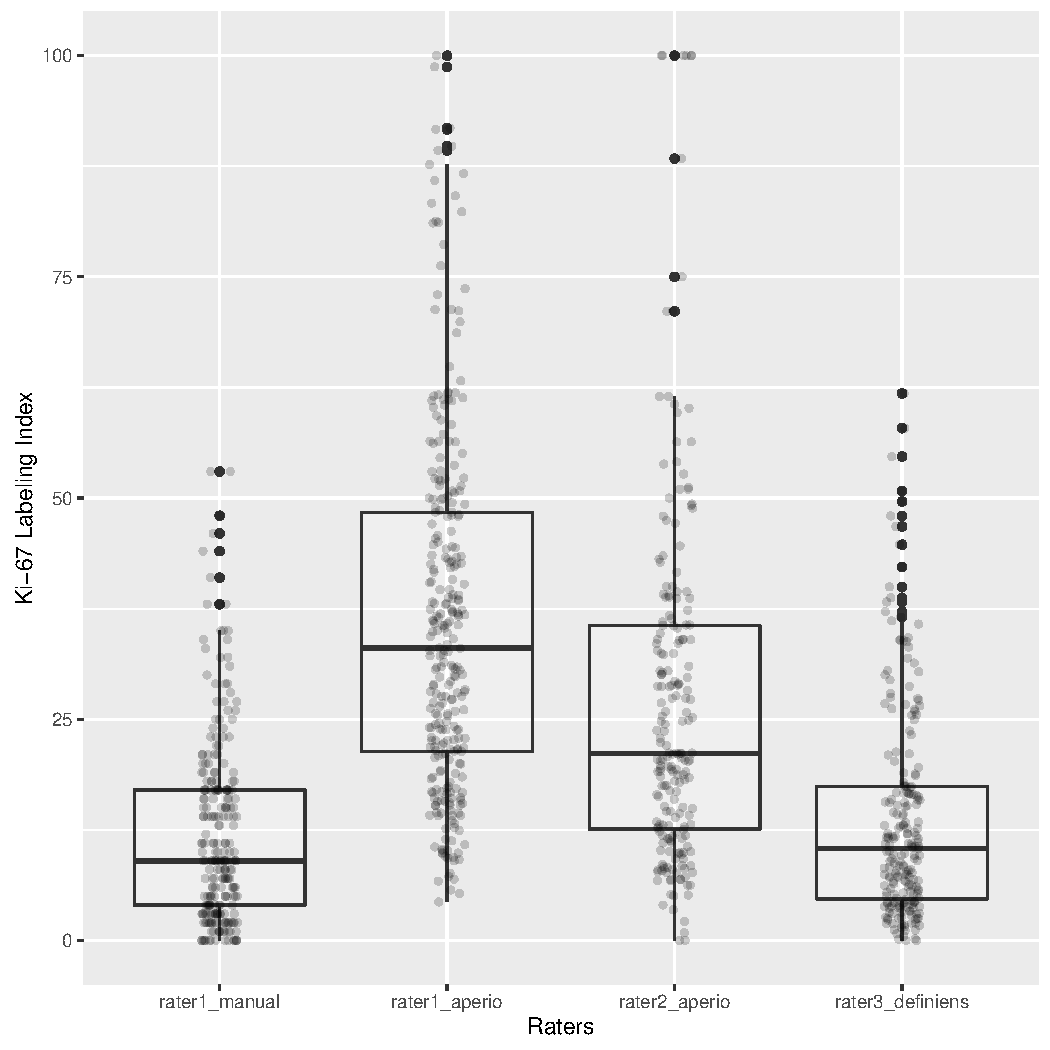
\includegraphics[width = 0.7\linewidth]{boxplot}
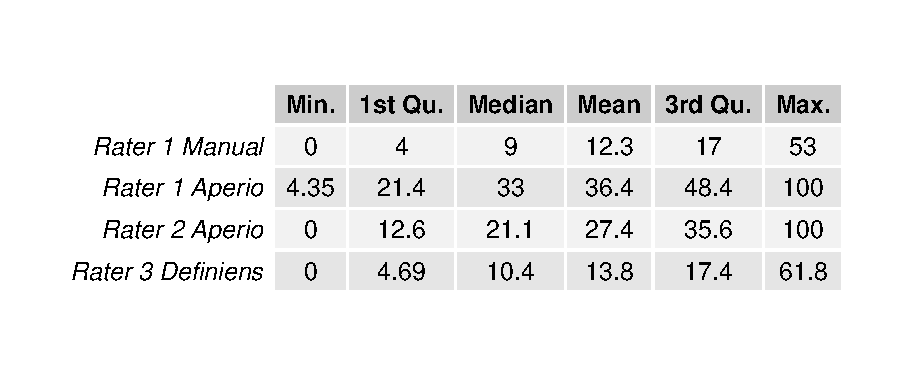
\includegraphics[width = \linewidth]{boxStat}

\centering
\caption{{\bf Boxplot and summary statistics}
Distribution of Ki-67 labeling index generated using manual assessment and DIA methods. Outliers are represented as darkened circles. Corresponding summary statistics quantitatively describes the boxplot.
}
\label{boxplot}
\end{figure}


\begin{figure}
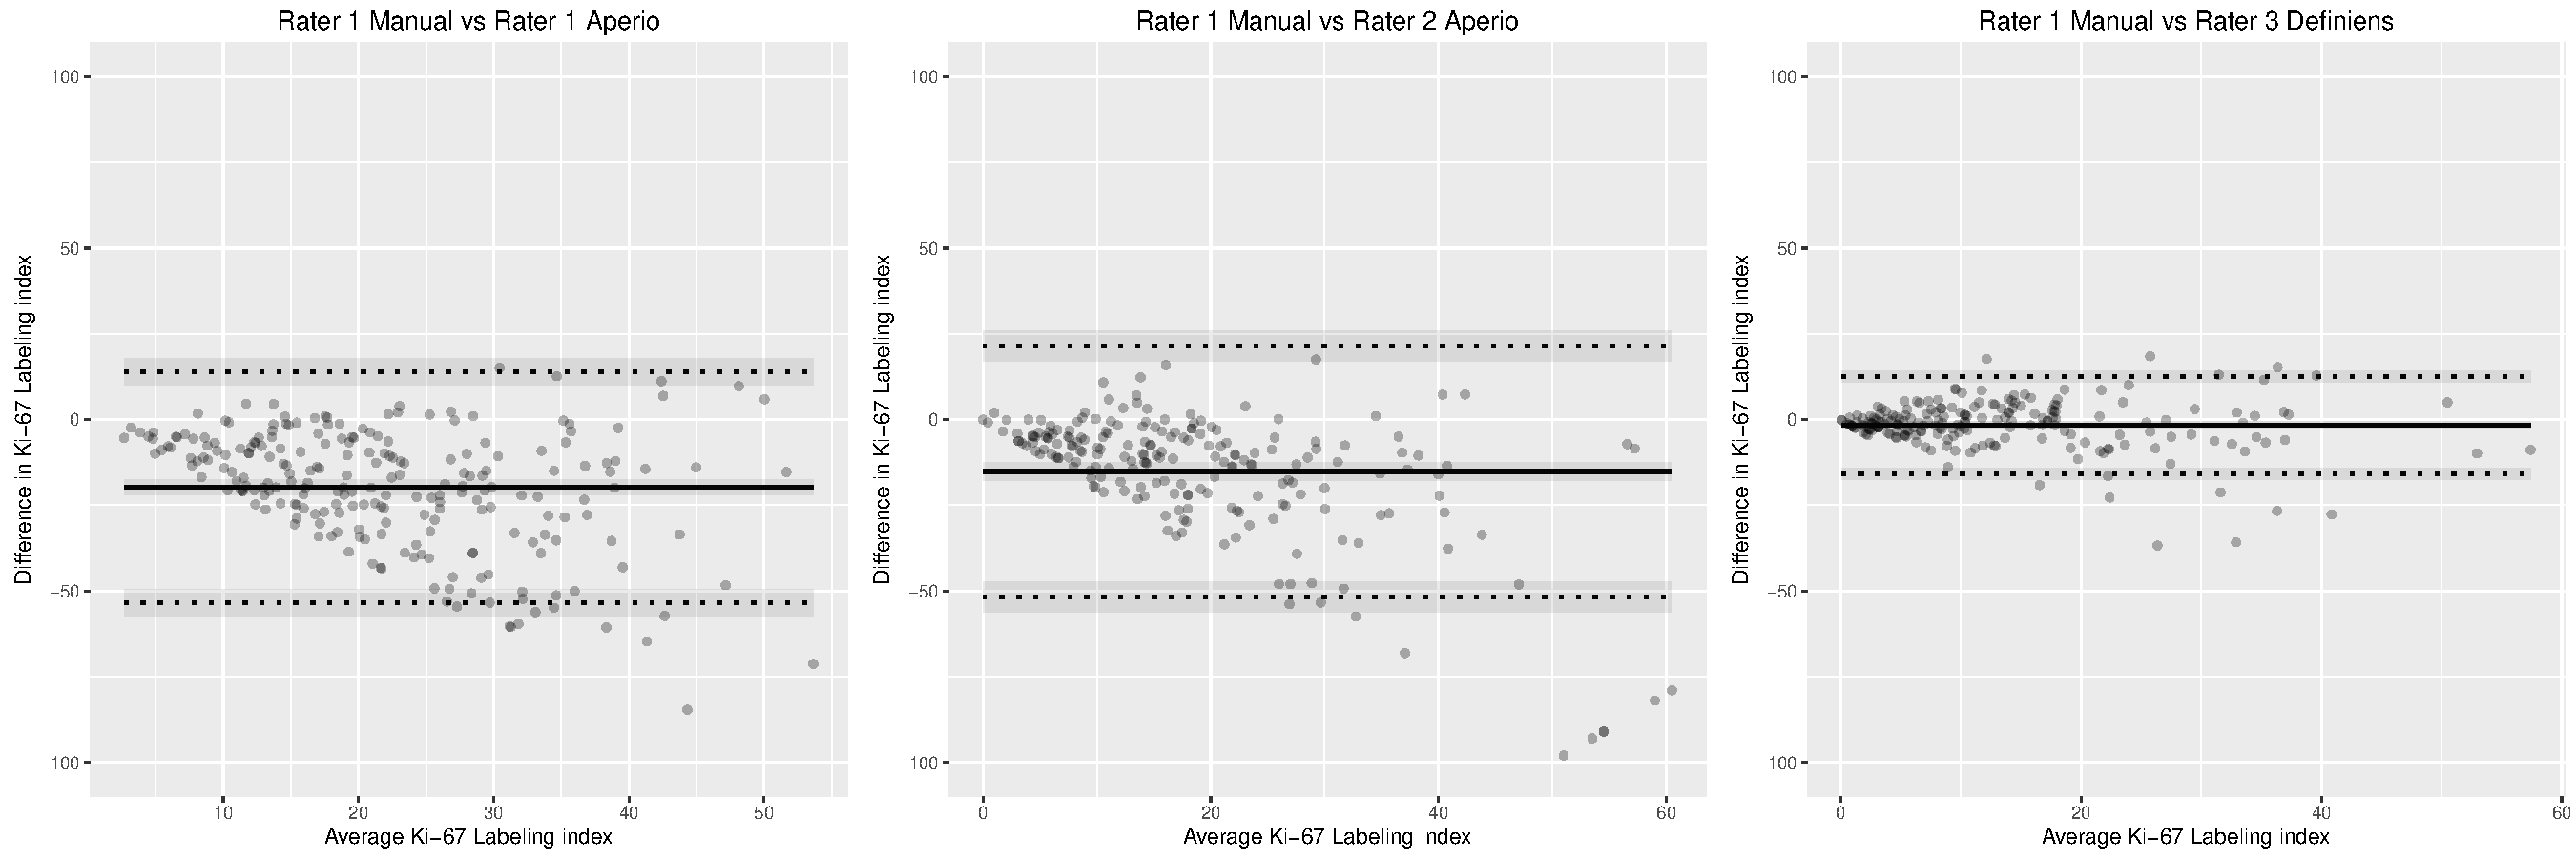
\includegraphics[width = \linewidth]{baplot}
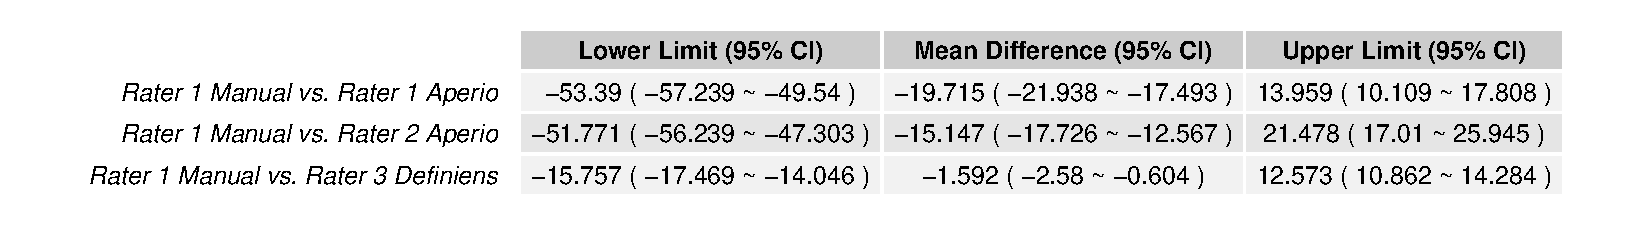
\includegraphics[width = \linewidth]{baStat}

\centering
\caption{{\bf Bland-Altman Plot}
Bias and agreement interval of manual reference score compared to results from DIA methods. Bland-Altman plot consists of a scatterplot, with each data point representing paired Ki-67 labeling index generated using methods in comparison. X axis is the average of paired measurement while the Y axis is the difference of paired measurement. Data points are flanked by dashed lines, which represent limits of agreement, within which 95\% of differences fall. Confidence intervals of mean difference as well as upper and lower limit of agreement are shown as grey area surrounding them. Statistics relevant to the plot are tabulated in the accompanying table.
}
\label{baplot}
\end{figure}


\begin{figure}
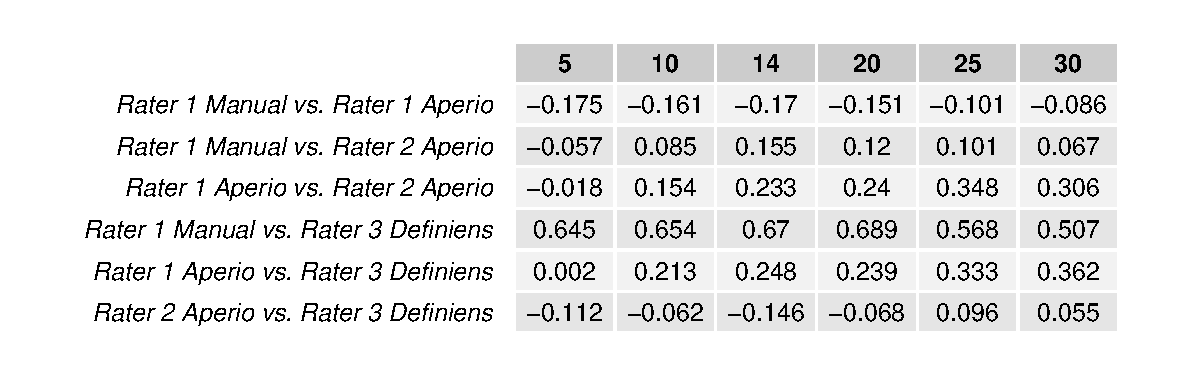
\includegraphics[width = \linewidth]{kappaStat}
\centering
\caption{{\bf Kappa statistics }
$\kappa$ calculated is a measurement of the extent that different rating instances correctly classify Ki-67 labeling index into Ki-67 low and Ki-67 high based on a selection of cut-offs, namely 5\%, 10\%, 14\%, 20\%, 25\%, 30\%.
}
\label{kappaStat}
\end{figure}




\end{document}
